
\chapter{Experiments}
\label{chp:exp}

\hspace{0.1in}
\section{Data Sets and Experimental Settings} \label{sec:DataSets}
We evaluate the proposed method on four data sources:
Netflix\footnote{http://www.netflix.com},
Douban,
IMDB\footnote{http://www.imdb.com},
and Wikipedia\footnote{http://en.wikipedia.org} user editing records.
The Netflix rating data contains more than $100$ million ratings with values in $\{1, 2, 3, 4, 5\}$, which are given by more than $4.8\times 10^5$ users
on around $1.8\times 10^4$ movies.
Douban contains movie, book and music recommendations, with rating values also in $\{1, 2, 3, 4, 5\}$.
IMDB hyperlink graph is employed as a measure of similarity between movies.
In the graph, each movie builds links to its $10$ most similar movies.
%The value $1$ is used to denote the top $10$ most similar movies for each movie in the movie-to-movie matrix.
The Wikipedia user editing records provide a $\{0, 1\}$ indicator of whether a user concerns or not about a certain movie.

The data sets used in the experiments are described as follows. For Netflix, to retain the original features of the users while keeping the size of the data set suitable for the experiments, we sampled a subset of $10,000$ users.
In Douban data sets, we obtained $1.2 \times 10^6$ ratings on $7.5 \times 10^3$ music, $ 5.8 \times 10^5 $ ratings on $3.5 \times 10^3 $ books, and $1.4 \times 10^6 $ ratings on $8 \times 10^3$ movies, given by $1.1 \times 10^4 $ users.
For both the IMDB data set and the Wikipedia data set, we filtered them by matching the movie titles in both the Netflix and the Douban Movie data sets. After pre-processing, the IMDB hyperlink data set contains $\sim 5 \times 10^3$ movies. The Wikipedia user editing records data set has $1.1 \times 10^6$ editing logs by $8.5 \times 10^3$ users on the same $\sim 5 \times 10^3$ movies as IMDB data set.
To present our experiments, we use the shorthand notations listed in Table \ref{tbl:notationDataset} to denote the data sets.


%%%%%%%%%%%%%%%%%%%%%%%%%%%-=Table1=-%%%%%%%%%%%%%%%%%%%%%%%%

\begin{table}[!tbp]
\caption{Datasets in our experiments.}
\label{tbl:notationDataset}
\begin{Large}
\begin{center}
\begin{tabular}{ c | c | c |c}
\hline\hline
Notation & Data Set & Data Type & Instances No. \\
\hline \hline
D1 & Douban Music & Rating [1,5]& $1.2 \times 10^6$\\
D2 & Douban Book & Rating [1,5]& $5.8 \times 10^5$ \\
D3 & Douban Movie & Rating [1,5]& $1.4 \times 10^6$ \\
D4 & Netflix & Rating [1,5]& $1.8 \times 10^4$\\
D5 & Wikipedia & Editing Log & $1.1 \times 10^6$\\
D6 & IMDB & Hyperlink & $5.0 \times 10^3$\\
\hline\hline
\end{tabular}
\end{center}
\end{Large}
\end{table}
%%%%%%%%%%%%%%%%%%%%%%%%%%%%%%%%%%%%%%%%%%%%%%%%%%%%%%%%%%

We evaluate the proposed algorithm on five cross-domain recommendation tasks, as follows:
\begin{itemize}[noitemsep,topsep=0pt,parsep=0pt,partopsep=0pt]
\item The first task is to simulate the cross-domain collaborative filtering, using the Netflix data set. The sampled data is partitioned into two parts with disjoint sets of movies but identical set of users. One part consists of ratings given by $8,000$ movies with $1.6\%$ density, which serves as the source domain. The remaining $7,000$ movies are used as the target domain with different levels of sparsity density.
\item The second task is a real-world cross-domain recommendation, where the source domain is Douban Book and the target domain is Douban Movie. In this setting, the source and the target domains share the same user set but have different item sets.
\item The third task is on Netflix and Douban data. We extract the ratings on the $6,000$ shared movies from Netflix and Douban Movie. Then we get $4.9 \times 10^5$ ratings from Douban given by $1.2 \times 10^4$ users with density $0.7\%$, and $10^6$ ratings from Netflix given by $10^4$ users with density $1.7\%$. The goal is to transfer knowledge from Netflix to Douban Movie. In this task, item set is identical across domains but user sets are totally different.
\item The fourth task is to evaluate the effectiveness of the proposed algorithm under the context of multiple source domains. It uses both Douban Music and Douban Book as the source domains and transfer knowledge to Douban Movie domain.
\item The fifth task varies the type of source domains. It utilizes the Wikipedia user editing records and IMDB hyperlink graph, together with Douban Movie as the source domains to perform rating predictions on the Netflix movie data set.
\end{itemize}

For evaluation, because we adopt the error rate style objective function in our optimization, we calculate the Root Mean Square Error (RMSE) on the heldout $\sim 30\%$ of the target data:
\begin{eqnarray}
    RMSE &=& \sqrt{ \sum_{ (u, i, x_{ui}) \in T_E } (x_{ui} - \hat{x}_{ui})^2 / |T_E|} \nonumber
\end{eqnarray}
where $x_{ui}$ and $\hat{x}_{ui}$ are the true and predicted ratings, respectively, and $|T_E|$ is the number of test ratings.



%%%%%%%%%%%%%%%%%%%%%%%%%%%-=Table2=-%%%%%%%%%%%%%%%%%%%%%%%%
\begin{table*}[!tbp]
\caption{Prediction performance of STLCF and the baselines.}
\label{tbl:TLCF}
\begin{footnotesize}
\begin{center}
\begin{tabular}{ c || c || c || c c || c c || c  c } \hline\hline

% ************************************************************************************************
 \multirow{2}{*}{Datasets}
& \multirow{1}{*}{Source}
& \multirow{1}{*}{Target}
& \multicolumn{2}{c ||}{Non-TL}
& \multicolumn{2}{c ||}{Non-Selective TL}
& \multicolumn{2}{c }{\bf Selective TL}\\
\cline{4-9}
% \hline \hline
% \hline \hline
&sparseness
&sparseness
& \multicolumn{1}{c }{GPLSA}
& \multicolumn{1}{c||}{PMF}
& \multicolumn{1}{c }{TGPLSA}
& \multicolumn{1}{c||}{CMF}
& \multicolumn{1}{c }{STLCF(E)}
& \multicolumn{1}{c}{STLCF(EV)}\\
\hline \hline
D4(Simulated) & \multirow{3}{*}{1.6\%} & 0.1\% & 1.0012 & 0.9993 & 0.9652 & 0.9688 & 0.9596 & \textbf{0.9533} \\
\cline{3-9}
to      &                        & 0.2\% & 0.9839 & 0.9814 & 0.9528 & 0.9532 & 0.9468 & \textbf{0.9347} \\
\cline{3-9}
D4(Simulated) &                        & 0.3\% & 0.9769 & 0.9728 & 0.9475 & 0.9464 & 0.9306 & \textbf{0.9213} \\
\hline \hline
& \multirow{3}{*}{1.5\%} & 0.1\% & 0.8939 & 0.8856 & 0.8098 & 0.8329 & 0.7711 & \textbf{0.7568} \\
\cline{3-9}
D2 to D3&                        & 0.2\% & 0.8370 & 0.8323 & 0.7462 & 0.7853 & 0.7353 & \textbf{0.7150} \\
\cline{3-9}
&                        & 0.3\% & 0.7314 & 0.7267 & 0.7004 & 0.7179 & 0.6978 & \textbf{0.6859} \\
\hline \hline
& \multirow{3}{*}{1.7\%} & 0.1\% & 0.8939 & 0.8856 & 0.8145 & 0.8297 & 0.7623 & \textbf{0.7549} \\
\cline{3-9}
D4 to D3 &                        & 0.2\% & 0.8370 & 0.8323 & 0.7519 & 0.7588 & 0.7307 & \textbf{0.7193} \\
\cline{3-9}
&                        & 0.3\% & 0.7314 & 0.7267 & 0.7127 & 0.7259 & 0.6982 & \textbf{0.6870} \\
\hline \hline

\end{tabular}
\end{center}
\end{footnotesize}
\end{table*}
%%%%%%%%%%%%%%%%%%%%%%%%%%%%%%%%%%%%%%%%%%%%%%%%%%%%%%%%%%

\hspace{0.1in}
\section{STLCF and Baselines Methods}
We implement two variations of our STLCF method.
STLCF(E) is an STLCF method that only take training error into consideration when performing selective transfer learning.
STLCF(EV) not only considers training error, but also utilizes the empirical error variance.

To demonstrate the significance of our STLCF, we selected the following baselines:
\begin{itemize}
\item {\bf PMF}~\cite{/nips/SalakhutdinovM07} is a recently proposed method for missing value prediction. Previous work showed that this method worked well on the large, sparse and imbalanced data set.
\item {\bf GPLSA}~\cite{DBLP:conf/sigir/Hofmann03} is a classical non-transfer recommendation algorithm.
\item {\bf CMF}~\cite{/kdd/SinghG08} is proposed for jointly factorizing two matrices. Being adopted as a transfer learning technique in several recent works, CMF has been proven to be an effective cross-domain recommendation approach.
\item {\bf TGPLSA} is an uniformly weighted transfer learning model, which utilize all source data to help build the target domain model. It is used as one of the baselines because we adopt it as the base model of our boosting-based selective transfer learning framework.
\end{itemize}
Parameters for these baseline models are fine-tuned via cross validation.

\hspace{0.1in}
\section{Experimental Results}
\subsection{Performance Comparisons}
We test the performance of our STLCF methods against the baselines.
The results of the collaborative filtering tasks under three different target domain sparseness are shown in Table \ref{tbl:TLCF}.

First, we observe that the non-transfer methods, i.e. GPLSA and PMF, fail to give accurate predictions, especially when the target domain is severely sparse.
With the help of source domains, the (non-selective) transfer learning methods with equally weights on the source domains, like TGPLSA and CMF, can increase the accuracy of the rating predictions. And our selective transfer learning methods (i.e., STLCF(E) and STLCF(EV)) can do even better.
The fact that our STLCF outperforms others is expected because by performing the {\em selective} knowledge transfer, we use the truly helpful source domain(s), which is designed to handle the sparseness issue in CF problems.

Second, comparing the two non-selective TLCF methods with the other two selective TLCF methods, we observe that on the last two real world tasks (D2 to D3 and D4 to D3) when the target domain is extremely sparse (say 0.1\%), the improvement of accuracy achieved by our STLCF methods against the non-selective transfer learning methods is more significant than it does on the simulation data set based on Netflix (D4 to D4).
Notice that the inconsistency of the target domain and the source domains on the simulation data sets is much smaller than that on the real-world cases. The experiment results show that our STLCF algorithm is effective in handling the inconsistency between the sparse target domain and the source domains.

Third, we notice that some factors, like empirical error variance, may affect the prediction. In Table \ref{tbl:TLCF}, we compare our two STLCF methods, i.e., STLCF(E) and STLCF(EV) when the target domain sparsity is $0.1\%$. We can find that on the task ``D2 to D3", i.e., Douban Book to Movie, STLCF(EV) is much better than STLCF(E). But on the task ``D4(Simulated) to D4(Simulated)", the improvement of STLCF(EV) is not so significant against STLCF(E). These observations may be due to the domain consistency.
For the tasks ``D4(Simulated) to D4(Simulated)", both the source and target entities are movie ratings from Netflix data set, while the task ``D2 to D3" tries to transfer the knowledge from a book recommendation system to the movie recommendation system, which may contain some domain specific items.
When the target domain is very sparse, i.e. the user's ratings on the items are rare, there are chances to get high prediction accuracy occasionally on the observed data with a bad model on the source domains that are inconsistent with target domain. In this case, it is important to consider the variance of empirical error as well. Comparing to STLCF(E), STLCF(EV), which punishes the large variance, can better handle the domain inconsistency in transfer learning, especially when the target domain is sparse.

\hspace{0.05in}
\subsection{Results on Long-Tail Users} \label{sec:long-tail}
%%%%%%%%%%%%%%%%%%%%%%%%%%%-=Table3=-%%%%%%%%%%%%%%%%%%%%%%%%%%%%%%%
\begin{table} [t]
\begin{LARGE}
\caption{Prediction performance of STLCF for Long-Tail Users on the D2 to D3 task.}
\label{tbl:tail}
\begin{center}
\begin{tabular}{l||c|| cc||cc}
\hline\hline
Ratings & \multirow{1}{*}{\multirow{2}{*}{Non-TL}} & \multicolumn{2}{c ||}{\multirow{2}{*}{Non-Selective TL}} & \multicolumn{2}{c}{\bf Selective TL}\\
%\cline{3-6}
per & & & & \multicolumn{2}{c} {\bf i.e. STLCF}\\
\cline{2-6}
user & GPLSA & TGPLSA & CMF & (E) & (EV)\\
\hline\hline
1-5   & 1.1942 & 0.9294 & 0.9312 & 0.8307 & \textbf{0.8216}\\\hline
6-10  & 0.9300 & 0.7859 & 0.7929 & 0.7454 & \textbf{0.7428}\\\hline
11-15 & 0.8296 & 0.7331 & 0.7390 & \textbf{0.7143} & 0.7150\\\hline
16-20 & 0.7841 & 0.7079 & 0.7113 & \textbf{0.7042} & 0.7050\\\hline
21-25 & 0.7618 & 0.6941 & 0.6947 & 0.6942 & \textbf{0.6910}\\\hline
26-30 & 0.7494 & 0.6918 & 0.6884 & 0.6917 & \textbf{0.6852}\\\hline
31-35 & 0.7370 & 0.6909 & 0.6911 & 0.6915 & \textbf{0.6818}\\\hline
36-40 & 0.7281 & 0.6896 & 0.6856 & 0.6907 & \textbf{0.6776}\\\hline
41-45 & 0.7219 & 0.6878 & 0.6821 & 0.6890 & \textbf{0.6740}\\\hline
46-50 & 0.7187 & 0.6881 & 0.6878 & 0.6800 & \textbf{0.6734}\\
\hline
\hline
\end{tabular}
\end{center}
\end{LARGE}
\end{table}
%%%%%%%%%%%%%%%%%%%%%%%%%%%%%%%%%%%%%%%%%%%%%%%%%%%%%%%%%%
To better understand the impact of STLCF with the help of the source domain, we conduct a fine-grained analysis on the performance improvement on Douban data sets, with Douban Book as source domain and Douban Movie as target domain.
The results on different user groups in the target domain are shown in Table \ref{tbl:tail}. In the table, method STLCF(E) does not punish the large variance of empirical error, while STLCF(EV) does.
%The overall data sparsity for the target domain is 0.4\%.
First, we observe that the STLCF models, i.e., STLCF(E) and STLCF(EV) can achieve better results on those long-tail users who have very few ratings in historical logs.
Such fact implies that our STLCF methods could handle the long-tail users that really need a fine-grained analysis when performing knowledge transfer from source domains.
Current CF models without any fine-grained analysis on the specific users usually fail to capture the preferences of the long-tail users, while our STLCF methods work well because they can selectively augment the weight of the corresponding source domain instances with respect to those long-tail cases at both instance level and domain level.
Second, STLCF(EV) works better than STLCF(E) on those non-long-tail users, i.e., with more than 25 ratings per user in the historical log. This is expected because users with more ratings can benefit more from the error variance analysis to avoid negative knowledge transfer.
%%%%%%%%%%%%%%%%%%%%%%%%%%%-=Table4=-%%%%%%%%%%%%%%%%%%%%%%%%%%%%%%%
\begin{table*}[t]
\caption{Prediction performance of STLCF with multiple source domains containing much irrelevant information.}
\label{tbl:mdomainshyb}
\begin{center}
\begin{tabular}{ c | c || c || c | c | c | c | c }
\hline\hline
\multicolumn{2}{c ||} {Source Domain: }  & None  & D3 & D3 \& D5 & D3 \& D6 & D5 \& D6 & D3 \& D5 \& D6\\
\hline\hline
 \multirow{1}{*}{Target} & 0.1\% & 0.9983 & $0.9789$& $0.9747$& $0.9712$& $0.9923$&$\textbf{0.9663}$\\
\cline{2-8}
 \multirow{1}{*}{(D4)} & 0.2\% & 0.9812 & $0.9625$& $0.9583$&$0.9572$ & $0.9695$ & $\textbf{0.9505}$\\
\cline{2-8}
 \multirow{1}{*}{sparseness} & 0.3\%& 0.9703 & $0.9511$& $0.9409$& $0.9464$& $0.9599$ &$\textbf{0.9383}$\\
\hline\hline
\end{tabular}
\end{center}
\end{table*}
%%%%%%%%%%%%%%%%%%%%%%%%%%%%%%%%%%%%%%%%%%%%%%%%%%%%%%%%%%


%%%%%%%%%%%%%%%%%%%%%%%%%%%-=Table5=-%%%%%%%%%%%%%%%%%%%%%%%%%%%%%%%
\begin{table}[!tbp]
\caption{Prediction performance of STLCF with multiple source domains (Douban).}
\label{tbl:mdomainsDB}
\begin{Large}
\begin{center}
\begin{tabular}{ c |c || c || c | c | c }
\hline\hline
\multicolumn{2}{c ||} {Source Domain:} & None & D1 & D2 & D1 \& D2\\
\hline\hline
\multirow{1}{*}{Target} & 0.1\% & 0.8856& $0.7521$ & $0.7568$ & $\textbf{0.7304}$\\
\cline{2-6}
\multirow{1}{*}{(D3)} & 0.2\% & 0.8323 & $0.7163$ & $0.7150$ & $\textbf{0.6904}$\\
\cline{2-6}
\multirow{1}{*}{sparseness} & 0.3\%& 0.7267 & $0.6870$ & $0.6859$ & $\textbf{0.6739}$\\
\hline\hline
\end{tabular}
\end{center}
\end{Large}
\end{table}
%%%%%%%%%%%%%%%%%%%%%%%%%%%%%%%%%%%%%%%%%%%%%%%%%%%%%%%%%%

\hspace{0.05in}
\subsection{STLCF with Multiple Source Domains} \label{sec:multSource}
We apply STLCF(EV) on the extremely sparse target movie domain, with two sets of source domains: one is composed of Douban Music and Douban Book, the other is composed of Douban Movie, IMDB hyperlink graph and Wikipedia user editing records. The results are in Table \ref{tbl:mdomainsDB} and Table \ref{tbl:mdomainshyb} respectively. We demonstrate our STLCF method can utilize multiple source domains of various types by handling the inconsistency between the target and the source domains.


First, for the Douban experiments shown in Table \ref{tbl:mdomainsDB},
we observe that comparing to only using either Douban Book or Douban Music as source domain, there are significant improvements when both of them are used.
The result is expected because each of the source domains has its own parts of effective information for the target domain.
For example, a user who show much interests in the movie ``The Lord of the Rings'' may have consistent preferences in its novel. In this case, with the help of more auxiliary sources, better results are expected.

Second, we explore the generalization of the choices of source domains by introducing domains like Wikipedia user editing records and IMDB hyperlink graph, which are not directly related to the target domain but still contain some useful information in helping the target task (Netflix rating prediction). The results are shown in Table~\ref{tbl:mdomainshyb}.
Comparing the results of the experiment that uses no source domain (non-transfer) to those that use source domains D5 \& D6, we observe that although the Wikipedia user editing records or IMDB hyperlink graph is not closely related to the target domain and can hardly be adopted as source domains by previous transfer learning techniques, our STLCF method can still transfer useful knowledge successfully.

In addition, comparing the results of the experiment that uses single source domain D3 to those that use source domains D3 \& D5, D3 \& D6, or D3 \& D5 \& D6, we find that the Wikipedia user editing records or IMDB hyperlink graph could provide some useful knowledge that is not covered by the related movie source domains. Despite of the noise and heterogeneous setting, our STLCF method can still utilize these source domains to help the target domain tasks. As we have discussed in Chapter \ref{chp:STLCF}, our STLCF performs selective transfer learning at both domain level and instance level.
On one hand, the domain level selective transfer can block the noisy information globally. As we can see, D5 \& D6 are noisy and therefore contain much data that are inconsistent with the observed data in the target domain, therefore the overall transfer of D5 \& D6 is penalized.
On the other hand, the instance level selective transfer learning can further eliminate the affections of those irrelevant source instances.

Above all, our STLCF is highly adaptive to utilize source domains that are relatively inconsistent with the target domain, even when the target domain is rather sparse.

\hspace{0.05in}
\subsection{Parameters Analysis of STLCF}
There are two parameters in our STLCF, i.e., the prediction error threshold $\tau$ and the empirical error variance weight $\gamma$.
Since $\tau$ and $\gamma$ are independent, we fix one and adjust another.

We fix the empirical error variance weight to be $\gamma=0.5$ and adjust the parameter $\tau$. Based on our results shown in Figure \ref{fig:tau1} and Figure \ref{fig:tau2} for two different transfer learning tasks, the model has good performance when $\tau$ is of order $10^{-2}$.
We also tuned the parameter $\gamma$, which balances the empirical error and its variance. We fix the prediction error threshold to be $\tau=0.03$ in tuning $\gamma$. As shown in Figure \ref{fig:gamma1} and Figure \ref{fig:gamma2}, when we vary the parameter $\gamma$ from $0$ to $1$ in two settings, the best choices of $\gamma$ are found to be around $0.4-0.5$.

\begin{figure}[t]
\centering
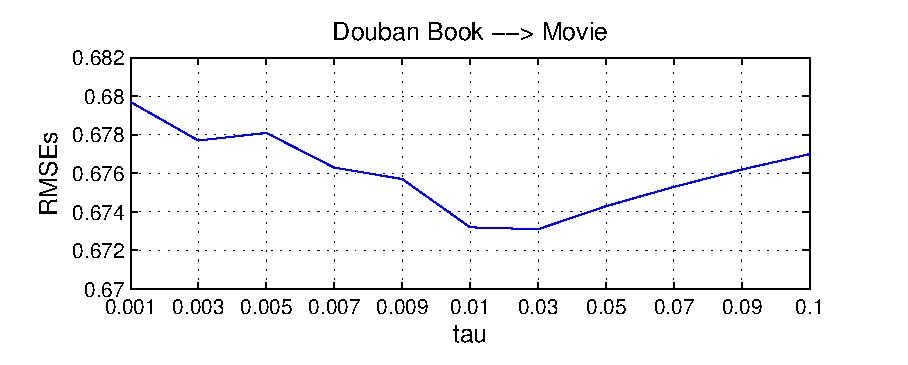
\includegraphics[width=6.5in]{fig/douban_tau.eps}
\caption{Change of the RMSEs with different $\tau$s. (Douban book to Movie)}\label{fig:tau1}
\end{figure}


\begin{figure}[t]
\centering
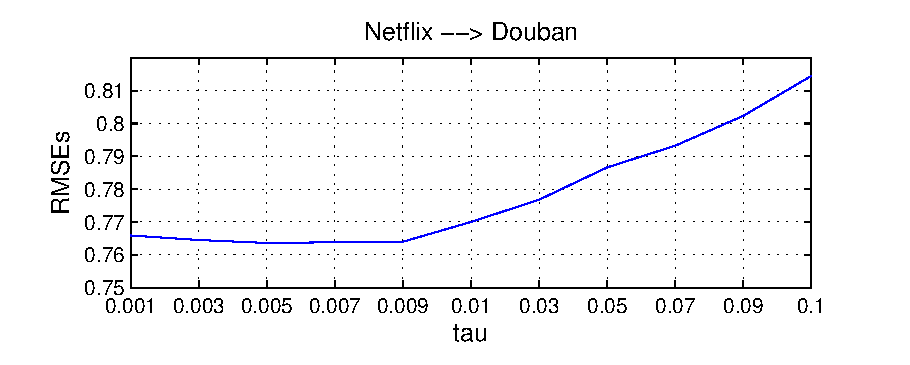
\includegraphics[width=6.5in]{fig/nf_tau.eps}
\caption{Change of the RMSEs with different $\tau$s. (Netflix to Douban Movie)}\label{fig:tau2}
\end{figure}


\begin{figure}[t]
\centering
\includegraphics[width=6.5in]{fig/douban_gamma.eps}
\caption{Change of the RMSEs with different $\gamma$s. (Douban book to Movie)}\label{fig:gamma1}
\end{figure}


\begin{figure}[t]
\centering
\includegraphics[width=6.5in]{fig/nf_gamma.eps}
\caption{Change of the RMSEs with different $\gamma$s. (Netflix to Douban Movie)}\label{fig:gamma2}
\end{figure}

\subsection{Convergence and Overfitting Test}
Figure \ref{fig:converge1} shows the RMSEs of STLCF(EV) as the number of weak learners changes on the Douban Book to Movie task. From the figure, we observe that STLCF(EV) converges well after 40 iterations. In Figure \ref{fig:converge2}, we can find that the corresponding $\alpha$ also converge to around 0.68 after 40 iterations as well. Empirically, we find STLCF converges in less than $50$ iterations.


\begin{figure}[t]
\centering
\includegraphics[width=6in]{fig/douban_learners.eps}
\caption{Change of the RMSEs when more and more weak learners join in the committee.}\label{fig:converge1}
\end{figure}

\begin{figure}[t]
\centering
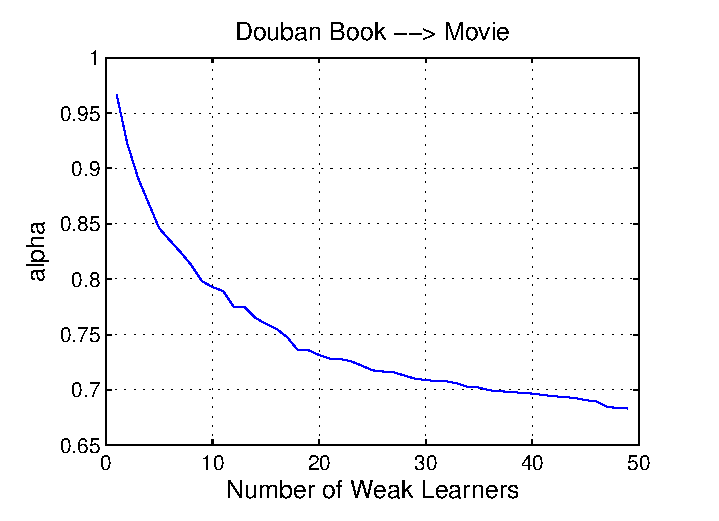
\includegraphics[width=6in]{fig/douban_alpha.eps}
\caption{Change of $\alpha$s when more and more weak learners join in the committee.}\label{fig:converge2}
\end{figure}

The number of latent topics of the base learner TGPLSA reflects the model's ability to fit training data. When we keep increasing the number of latent topics, the model tends to better fit the training data. But if the number of latent topics is too large, the model may suffer from overfitting.

We investigate the overfitting issue by plotting the training and testing RMSEs of the non-transfer learning model GPLSA, the non-selective transfer learning model TGPLSA and our selective transfer learning model STLCF(EV) over different numbers of latent topics in Figure \ref{fig:k}. The data sparsity for the target domain is around 0.3\%.

We can observe that comparing to our STLCF, the training RMSEs of GPLSA and TGPLSA decrease faster, while their testing RMSEs go down slower. When $k$ is about $50$, the testing RMSEs of GPLSA start to go up. And for TGPLSA, its testing RMSEs also go up slightly when $k$ is larger than $75$. But the testing RMSEs of our STLCF keep decreasing until $k=125$ and even when $k$ is larger than $125$, the raise of our STLCF's testing RMSEs is not obvious. Clearly when the target domain is very sparse, our STLCF method is more robust against the overfitting, by inheriting the advantage from boosting techniques and the fine-grained selection on knowledge transfer.

\begin{figure}
\begin{minipage}[t]{0.95\linewidth}
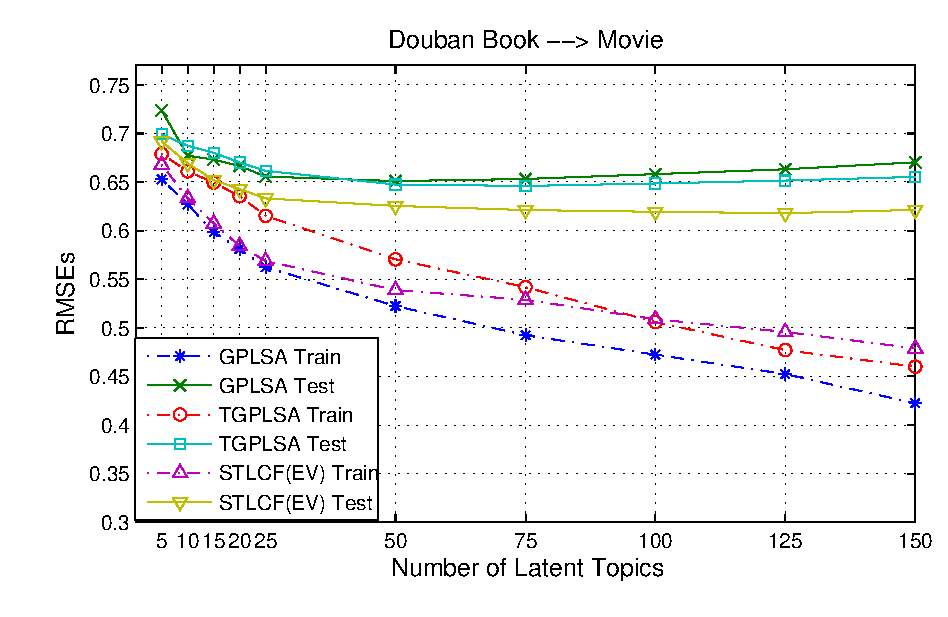
\includegraphics[width=6.5in]{fig/douban_k.eps}
\end{minipage}
\caption{Change of the RMSEs with different numbers of latent topics.}\label{fig:k}
\end{figure}
